\documentclass[a4paper,12pt,titlepage]{scrartcl}

%%%%%%%%%%%%%%%%%%%%%%%%%%%%%%%%%%%%%%%%%%%%%%%%%%%%%%%%%%%%%%%%%%%%%%%%%%%%%%%%%%%%%%%%%%%%%%%%%%%%%%%%%%%%%%%%%%%%%%%%%%%%%%%%%%%%%%%%%%%%%%%%%%%%%%%%%%%%%%%%%%%%%%%%%%%%%%%%%%%%%%%%%%%%%%%%%%%%%%%%%%%%%%%%%%%%%%%%%%%%%%%%%%%%%%%%%%%%%%%%%%%%%%%%%%%%
\usepackage[textwidth=125mm, textheight=195mm]{geometry}
\usepackage[portuguese]{babel}
\usepackage{graphicx}
\usepackage{amsmath}
\usepackage{amsfonts}
\usepackage{amsthm}
\usepackage{epstopdf}
\usepackage{listings}
\usepackage{color}
\usepackage[nottoc,numbib]{tocbibind}
\usepackage[colorlinks=true]{hyperref}



\geometry{verbose,a4paper,tmargin=20mm,bmargin=30mm,lmargin=15mm,rmargin=15mm}


\definecolor{codegreen}{rgb}{0,0.6,0}
\definecolor{codegray}{rgb}{0.5,0.5,0.5}
\definecolor{codepurple}{rgb}{0.58,0,0.82}
\definecolor{backcolour}{rgb}{0.95,0.95,0.92}

\lstdefinestyle{mystyle}{
    backgroundcolor=\color{backcolour},   
    commentstyle=\color{codegreen},
    keywordstyle=\color{magenta},
    numberstyle=\small,
    stringstyle=\color{codepurple},
    basicstyle=\ttfamily\footnotesize,
    breakatwhitespace=false,         
    breaklines=true,                 
    captionpos=b,                    
    keepspaces=true,                 
    numbers=left,                    
    numbersep=5pt,                  
    showspaces=false,                
    showstringspaces=false,
    showtabs=false,                  
    tabsize=3,
    showlines = true
}

\lstset{style=mystyle}

\begin{document}

\newcommand{\wk}{\mbox{$\,<$\hspace{-5pt}\footnotesize )$\,$}}




\numberwithin{equation}{section}
\newtheorem{teo}{Theorem}
\newtheorem{lemma}{Lemma}

\newtheorem{coro}{Corollary}
\newtheorem{prop}{Proposition}
\theoremstyle{definition}
\newtheorem{definition}{Definition}
\theoremstyle{remark}
\newtheorem{remark}{Observação}

\newtheorem{scho}{Scholium}
\newtheorem{open}{Question}
\newtheorem{example}{Example}
\numberwithin{example}{section}
\numberwithin{lemma}{section}
\numberwithin{prop}{section}
\numberwithin{teo}{section}
\numberwithin{definition}{section}
\numberwithin{coro}{section}
\numberwithin{figure}{section}
\numberwithin{remark}{section}
\numberwithin{scho}{section}

\bibliographystyle{abbrv}

\begin{titlepage}
\begin{center}
\vspace*{1cm}
\textbf{\large Algoritmos de vizinhos mais próximos aproximados}\\
\vspace*{2cm}

\end{center}
\textbf{Disciplina: TCC00288}\\
\textbf{Professora: Luiz André Portes Paes Leme}
\begin{center}
\vspace*{6cm}
Barbara Keren Nascimento C. Guarino \\
Bruna de Assunção Santos\\
Gabriel Gavazzi Felix\\
Gabriel Ramalho Braga \\
Tatiana Machado Brito dos Santos\\
Vitor Balestro Dias da Silva

\vspace*{6cm}


\includegraphics[scale=0.2]{logo.png}

\end{center}
\end{titlepage}

\section{Descrição do problema}

Informalmente, o problema dos $k$ vizinhos mais próximos consiste em encontrar os $k$ vetores de um dado conjunto $S$ que estão mais próximos de um dado vetor $v$. Formalmente, sejam $k,n \in \mathbb{N}$, $S \subseteq \mathbb{R}^n$ e $v \in \mathbb{R}^n$. Assuma que $S$ é um conjunto finito com $m$ elementos, onde $m \geq k$, e seja $d$ uma distância em $\mathbb{R}^n$. Considere a ordenação
\begin{align*} S = \{v_1,\ldots,v_m\}
\end{align*} 
onde $d(v_j,v) \geq d(v_i,v)$ sempre que $j > i$ (isto é, $S$ está ordenado pela distâncias a $v$). Desejamos encontrar o conjunto
\begin{align*} \mathrm{NN}_k(v,S,d) := \{v_1,\ldots,v_k\}. 
\end{align*}
Não é difícil implementar um algoritmo computacional que forneça uma solução exata para este problema. Entretanto, a depender do tamanho de $S$, tal solução seria computacionalmente cara. De fato, é preciso calcular as distâncias dos elementos de $S$ a $v$ e, em seguida, ordená-las.

Desta forma, o desafio é desenvolver e implementar algoritmos que encontrem \emph{aproximadamente} os $k$ vizinhos mais próximos. Em linhas gerais, o objetivo é obter \emph{boas} aproximações com \emph{baixo} custo de execução. Note que os adjetivos em itálico referem-se a propriedades que são, ao menos em alguma medida, subjetivas. 

Em uma descrição de alto nível, um \emph{algoritmo de vizinhos mais próximos aproximados} (vamos chamá-lo de $\pi$) consiste me duas etapas: \\

\noindent\textbf{(i)} uma fase de \emph{pré-processamento}, em que são construídas estruturas de dados para $S$;\\

\noindent\textbf{(ii)} a fase de processamento em que, dados um número $k \in \mathbb{N}$ e um vetor $v$, é retornado um conjunto $\mathrm{ANN}_k(v,S,d)=\{w_1,\ldots,w_{k^*}\} \subseteq S$ (com $k \leq k^*$) de vizinhos mais próximos aproximados de $v$. \\

Em linhas gerais, a qualidade da aproximação obtida é mensurada comparando o conjunto aproximado obtido $\mathrm{ANN}_k(\pi,v,S,d)$ com a solução exata (ordenada) $\mathrm{NN}(v,S,d) = \{v_1,\ldots,v_k\}$. Formalmente, definimos o \emph{recall} da solução aproximada como
\begin{align*} \mathrm{recall}(\pi) = \frac{\Big|\Big\{w \in \mathrm{ANN}_k(\pi,v,S,d) \colon d(w,v) \leq d(w,v_k)\Big\}\Big|}{k},
\end{align*}
onde denotamos por $|A|$ a quantidade de elementos do conjunto $A$. Nesta definição, estamos contando quantos vetores da solução aproximada têm distância para $v$ mais próxima do que $v_k$, que é o último vetor da solução exata ordenada. 

Note que para calcular o recall, precisamos apenas de $d(w,v_k)$. Assim, esta distância será chamada \emph{distância de referência} a partir de agora. 

\section{Tabelas}

Consideramos o problema sobre um conjunto $S$ de $1000000$ de vetores em $\mathbb{R}^{128}$ com $k = 100$. No banco de dados, temos as seguintes tabelas:\\\

\noindent\textbf{(i) object:} contém os vetores do conjunto $S$. Portanto, é uma tabela com 1000000 de linhas, em que cada linha é um vetor de 128 coordenadas;\\

\noindent\textbf{(ii) tquery:} contém um conjunto de 10000 casos de teste, para os quais a solução exata é conhecida ; \\

\noindent\textbf{(iii) neighbor:} contém as soluções exatas para os vetores da tabela \textbf{tquery}. Assim, é uma tabela de 10000 linhas em que cada linha é um vetor de 100 coordenadas.\\

Para o que segue, denote por $\mathrm{tabela}[j]$ a $j$-ésima linha de uma tabela, e por $\mathrm{vetor}[j]$ a j-ésima coordenada de um vetor. Para cada $1 \leq j \leq 10000$, o vetor $\mathrm{neighbor}[j]$ contém os \emph{índices} dos $100$ vetores da tabela object que estão (ordenadamente) mais próximos o vetor $\mathrm{tquery}[j]$. Estes índices se referem à tabela object. Por exemplo, se
\begin{align*} \mathrm{neighbor}[10] = (20,12,14,\ldots),
\end{align*}
então os vetores de object mais próximos do vetor $\mathrm{tquery}[10]$ são 
\begin{align*}\mathrm{object}[20], \,\mathrm{object}[12],\, \mathrm{object}[14],\, \ldots 
\end{align*}

\section{Pré-processamento}

Na fase de pré-processamento, primeiro executamos um algoritmo de \emph{clusterização} de $S$. Para este fim, usamos o algoritmo \emph{KMeans} da biblioteca \emph{scikit} da linguagem \emph{Python}. Informalmente, este algoritmo agrupa os vetores de $S$ em $k$ conjuntos de vetores pŕoximos entre si, e retorna os \emph{centróides} destes conjuntos (pense no centróide como um vetor que é, de alguma forma, central dentro do conjunto). Consideramos $k = 128$, e isso significa que o algoritmo retornará uma tabela com 128 vetores de $S$ (os \emph{centróides}). Estes vetores estão armazenados na tabela \textbf{sight}. Esta tabela tem duas colunas: \textbf{id}, que é a chave primária (inteiros sequenciais) e \textbf{centroid}, que armazena o centróide correspondente (vetor de inteiros). 

O próximo passo é criar uma tabela que informe o centróide mais próximo de cada vetor da tabela \textbf{object} (e a distância do vetor ao seu centróide mais próximo). Assim, dado um vetor \textbf{query}, podemos, por exemplo, restringir a busca aos vetores cujo centróide mais próximo é o centróide mais próximo de \textbf{query}. A tabela que guarda estas informações é chamada \textbf{closer$\_$centroids}, e o código para gerá-la é exibido abaixo. Vale notar que esta etapa é custosa. Note que a chamada da função recebe como parâmetros a quantidade de vetores de \textbf{object} para os quais o centróide mais próximo será calculado e um valor de \emph{offset}. Para evitar esgotamento de memória principal, dividimos a tabela rodando a função para cada uma de suas partes. Em um notebook de categoria intermediária, cada execução para 100000 vetores levou em torno de 4 minutos. \\

\begin{lstlisting}[caption = Obtendo a tabela de centróides mais próximos, label = closcent]
CREATE TYPE tuple AS (ind int, dist double precision);

CREATE OR REPLACE FUNCTION get_closer_centroids(qtd int,offs int) RETURNS void AS $$
DECLARE
	object_line record;
	sight_line record;
	distances_vector tuple[];
	current_tuple tuple;
	dist double precision;
	min_dist double precision;
	i int;
	ind int;
BEGIN
	FOR object_line IN SELECT * FROM object ORDER BY id LIMIT qtd OFFSET offs LOOP
		FOR sight_line IN SELECT * FROM sight_ LOOP
			dist = euclidean_distance(object_line.features,sight_line.centroid);
			current_tuple = (sight_line.id,dist);
			distances_vector[sight_line.id] = current_tuple;
		END LOOP;
		min_dist = distances_vector[1].dist;
		ind = 1;
		FOR i in 1..128 LOOP
			IF (distances_vector[i].dist < min_dist) THEN
				min_dist = distances_vector[i].dist;
				ind = distances_vector[i].ind;
			END IF;
		END LOOP;
		INSERT INTO closer_centroids VALUES (object_line.id,ind, min_dist);
	END LOOP;
END;
$$ LANGUAGE plpgsql;

\end{lstlisting}
\vspace{5mm}

O esquema lógico das tabelas criadas na etapa de pré-processamento está no Appêndice \ref{app0}


\section{Método 1: busca por regiões parametrizadas}

Este método de busca dos 100 vetores mais próximos de um vetor \textbf{q} é como segue:\\

\noindent$\bullet$ \textbf{Passo 1:} encontramos o centróide \textbf{c} mais próximo de \textbf{q};\\

\noindent$\bullet$ \textbf{Passo 2:} computamos a distância $d$ de \textbf{q} para \textbf{c};\\

\noindent$\bullet$ \textbf{Passo 3:} escolhemos parâmetros $0 < \alpha < 1$, $\beta > 1$ e $0 < \gamma < 1$ e, dentre os vetores $v \in S$ (tabela \textbf{object}) cujo centróide mais próximo é \textbf{c}, encontramos aqueles que satisfazem:\\

\noindent\textbf{(i)} $\alpha d < d(v,\mathbf{c}) < \beta d$, e \\

\noindent\textbf{(ii)} $\gamma < \mathrm{cos}(v-\mathbf{c},\mathbf{q}-\mathbf{c}) < 1$.\\

Isto é, consideramos a interseção entre a coroa circular com centro em \textbf{c} e raios $\alpha d$ e $\beta d$ (interno e externo, respectivamente) com o cone de vetores $w$ tais que o cosseno do ângulo entre $w - \mathbf{c}$ e $\mathbf{q} - \mathbf{c}$ é menor do que $\gamma$. Veja a Figura \ref{figmetodo1} para uma ilustração da região considerada.

\begin{figure}[h]
\centering
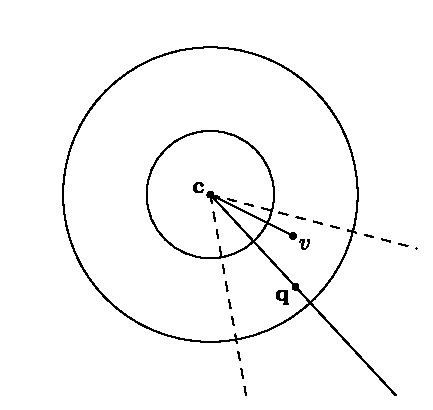
\includegraphics{metodo1.eps}
\caption{Ilustração em duas dimensões do método 1.}
\label{figmetodo1}
\end{figure}

Para fins de simplicar a notação, a partir de agora vamos denotar por $S_{\mathbf{c}}$ o subconjunto dos vetores de $S$ que têm \textbf{c} como centróide mais próximo. 

Aqui, vale um comentário sobre a eficiência deste algoritmo. A tabela \textbf{closer$\_$centroids} já fornece a distância entre cada vetor $v \in S_{\mathbf{c}}$ cujo centróide \textbf{c}. Assim, nenhuma distância será calculada no passo 3. Mais ainda, lembre-se de que o valor do cosseno entre $v-\mathbf{c}$ e $\mathbf{q}-\mathbf{c}$ é computado pela fórmula
\begin{align*} \mathrm{cos}(v-\mathbf{c},\mathbf{q}-\mathbf{c}) = \frac{\langle v-\mathbf{c},\mathbf{q}-\mathbf{c}\rangle}{||v-\mathbf{c}||\,||\mathbf{q}-\mathbf{c}||} = \frac{\langle v-\mathbf{c},\mathbf{q}-\mathbf{c}\rangle}{d(v,c)\cdot d}
\end{align*}
A norma de $v - \mathbf{c}$ é igual à distância entre $v$ e \textbf{c} e, portanto, não precisará ser calculada. A norma de $\mathbf{q} - \mathbf{c}$ é igual à $d$, que foi calculado no passo 1. Daí, apenas o produto interno deverá ser computado. Ou seja, para cada $v \in S_{\mathbf{c}}$, o produto interno $\langle v-\mathbf{c},\mathbf{q}-\mathbf{c}\rangle$ será calculado. Para calcular cada um destes produtos internos, são realizadas 128 multiplicações dentro de um \emph{loop} que atualiza uma soma. \\

\begin{remark} Note que para encontrar o conjunto $S_{\mathbf{c}}$, teremos que executar a seguinte consulta:\\

\begin{lstlisting}[caption = Encontrando $S_{\mathbf{c}}$, label = sc]

SELECT * FROM closer_centroids WHERE closer_centroid_ind = id(c);
   
\end{lstlisting}
\vspace{5mm}
onde id(c) é a chave do centróide \textbf{c} (na tabela \textbf{sight$\_$}, é claro). Para otimizar estas consultas, criamos um índice na tabela \textbf{closer$\_$centróides}:\\


\begin{lstlisting}[caption = Índice na chave do centróide mais próximo, label = indice]

CREATE INDEX closer_centroid_idx ON closer_centroids (closer_centroid_ind);

\end{lstlisting}
\vspace{5mm}
\end{remark}

Esta consulta, que é feita originalmente sobre uma tabela com 1000000 de entradas, leva 60 milisegundos, em média (novamente, em um notebook pessoal de nível intermediário). 

Vamos agora à implementação do método. Primeiro, notamos que o método depende de três parâmetros. Ao início da execução, esta tripla de parâmetros será armazenada em uma tabela (\textbf{method1$\_$parameters$\_$key}). Desta forma, cada tripla de parâmetros pode ser referênciada por uma chave primária. Se a tripla de parâmetros já estiver cadastrada, então ela não será recadastrada.

Os resultados encontrados (isto é, os 100 vetores mais próximos aproximados) serão armazenados na tabela \textbf{result$\_$table$\_$method1}). Cada linha desta tabela armazenará a chave da tripla de parâmetros considerada, o índice do vetor \textbf{query}, o vetor resultado e a distância do vetor resultado para o vetor \textbf{query} (esta distância será usada para computar o \emph{recall} mais tarde). Se a tabela já contiver resultados para a chave (tripla de parâmetros, vetor query) considerados, a execução será abortada (para evitar duplicidade). 

O código segue abaixo:\\

\begin{lstlisting}[caption = O algoritmo do Método 1., label = algmetodo1]
CREATE OR REPLACE FUNCTION ann_method1(query_vector_id int, alpha double precision, beta double precision, gamma double precision) 
RETURNS void AS $$
DECLARE
	query_vector int[]; -- q
	closer_centroid int[]; -- c
	diff_centroid_query int[]; -- q - c
	diff_candidate_centroid int[]; -- v - c
	closer_centroid_index int;
	candidate_vector int[]; -- v
	dist_query_centroid double precision; -- ||q-c|| = d
	dist_candidate_centroid double precision; -- ||v-c||;
	dist_candidate_query double precision; -- ||v-q||;
	inner_product double precision;
	cosine double precision;
	counter int;
	n int;
	parameters_key_value int;
	reference_dist double precision;
	line_ record;
	i int;
BEGIN
	n = (SELECT COUNT(*) FROM method1_parameters_key AS par WHERE par.alpha_ = alpha AND par.beta_ = beta AND par.gamma_ = gamma); 
	IF (n = 0) THEN
		INSERT INTO method1_parameters_key (alpha_,beta_,gamma_) VALUES (alpha,beta,gamma);
		parameters_key_value = (SELECT par.id FROM method1_parameters_key AS par WHERE par.alpha_ = alpha AND par.beta_ = beta AND par.gamma_ = gamma); 
		n = (SELECT COUNT(*) FROM result_table_method1 WHERE parameter_key_value = parameters_key_value AND query_vector_id_ = query_vector_id);
		IF (n != 0) THEN
			RAISE EXCEPTION 'The function was already computed for this query vector and these parameter values';
		END IF;
	END IF;
	
	SELECT query INTO query_vector FROM tquery WHERE id = query_vector_id;
	closer_centroid_index = get_closer_centroid_tquery(query_vector_id);
	SELECT centroid INTO closer_centroid FROM sight_ WHERE id = closer_centroid_index;
	dist_query_centroid = euclidean_distance(closer_centroid,query_vector);
	FOR i IN 1..128 LOOP
		diff_centroid_query[i] = query_vector[i] - closer_centroid[i];
	END LOOP;
	counter = 0;
	FOR line_ IN SELECT * FROM closer_centroids WHERE closer_centroid_ind = closer_centroid_index LOOP
		SELECT features INTO candidate_vector FROM object WHERE id = line_.id;
		dist_candidate_centroid = euclidean_distance(candidate_vector,closer_centroid);
		dist_candidate_query = euclidean_distance(candidate_vector, query_vector);
		FOR i IN 1..128 LOOP
		diff_candidate_centroid[i] = candidate_vector[i] - closer_centroid[i];
		END LOOP;
		IF (dist_candidate_centroid > alpha * dist_query_centroid AND dist_candidate_centroid < beta * dist_query_centroid) THEN
			inner_product = get_inner_product(diff_centroid_query, diff_candidate_centroid) :: double precision;
			cosine = inner_product/(dist_candidate_centroid * dist_query_centroid);
			IF (cosine > gamma AND cosine < 1) THEN
				INSERT INTO result_table_method1(parameter_key_value,query_vector_id_,vector,distance) VALUES
					(parameters_key_value,query_vector_id,candidate_vector,dist_candidate_query);
				counter = counter + 1;
			END IF;
		END IF;
	END LOOP;
	IF counter > 100 THEN
		reference_dist = (SELECT distance FROM result_table_method1 AS r 
		WHERE r.parameter_key_value = parameters_key_value AND
			  r.query_vector_id_ = query_vector_id 
		ORDER BY distance
		LIMIT 1
		OFFSET 99);
		
		DELETE FROM result_table_method1 AS r
		WHERE r.parameter_key_value = parameters_key_value AND
			  r.query_vector_id_ = query_vector_id AND
			  distance > reference_dist;
	END IF;
	
END;
$$ LANGUAGE plpgsql;

\end{lstlisting}
\vspace{5mm}

\section{Calculando o \textit{recall}}

Para calcular o \emph{recall} de uma determinada execução, primeiro obtemos a distância referência correspondente (através da tabela \textbf{neighbor}). Usamos a função explicitada abaixo para calcular a distância de referência do $j$-ésimo vetor da tabela \textbf{object} (isto é, o vetor cujo id é $j$).\\

\begin{lstlisting}[caption = Calculando a distância de referência., label = refdist]
CREATE OR REPLACE FUNCTION get_reference_distance(j int) RETURNS double precision AS
$$
DECLARE
	query_vector int[];
	neighbors_vector int[];
	index_ int;
	reference_vector double precision [];
	
BEGIN 
	query_vector := (SELECT query FROM tquery WHERE id = j);
 	neighbors_vector := (SELECT neighbors FROM neighbors WHERE id = j);
	index_ := neighbors_vector[100];
	reference_vector := (SELECT features FROM object WHERE id = index_);
	
	RETURN euclidean_distance(query_vector,reference_vector);
	
END;
$$ LANGUAGE plpgsql;

\end{lstlisting}
\vspace{5mm}

O algoritmo exato para computar o \emph{recall} depende do método adotado. Para o Método 1, a tabela de resultados (\textbf{result$\_$table$\_$method1} já fornece a distância de cada vetor da solução ao vetor \textbf{query}. Assim, usamos a seguinte função:\\

\begin{lstlisting}[caption = Calculando o \emph{recall} no Método 1., label = recallfunc]
CREATE OR REPLACE FUNCTION get_recall_method1(query_vector_index int, parameters_key int) RETURNS double precision AS
$$
DECLARE
	i int;
	query_vector int[];
	result_vector double precision[];
	reference_distance double precision;
	hit_count int;
	dist double precision;
	line_ record;
	recall_ double precision;
BEGIN
	hit_count = 0;
	reference_distance = get_reference_distance(query_vector_index);
	FOR line_ IN (SELECT * FROM result_table_method1 WHERE parameter_key_value = parameters_key AND query_vector_id_ = query_vector_index) LOOP
		IF(line_.distance <= reference_distance) THEN
			hit_count = hit_count + 1;
		END IF;
	END LOOP;
	recall_ = hit_count :: double precision / 100;
	INSERT INTO recall_table_method1(query_vector_id,parameters_key_,recall) VALUES
		(query_vector_index,parameters_key,recall_);
	RETURN recall_;
END;
$$ LANGUAGE plpgsql;

\end{lstlisting}
\vspace{5mm}

Observe que esta função calcula o \emph{recall} obtido para determinado vetor (da tabela \textbf{tquery}) com um determinado conjunto de parâmetros ($\alpha$, $\beta$ e $\gamma$). Assim, podemos rodar o algoritmo do Método 1 para diversos vetores de \textbf{tquery} e diversas combinações de parâmetros antes de computar o \emph{recall} de cada combinação. Isto torna mais conveniente obter estatísticas de eficiência do método, como ficará claro mais tarde. 

Para computar e armazenar o \emph{recall} de todos os vetores de \textbf{tquery} para determinado conjunto de parâmetros, executamos a função:\\

\begin{lstlisting}[caption = Computando o \emph{recall} para todos os vetores de \textbf{tquery}., label = recalltodos1]
CREATE OR REPLACE FUNCTION get_recall_for_all(parameters_key int) RETURNS void AS
$$
DECLARE
	alpha double precision;
	beta double precision;
	gamma double precision;
BEGIN
	alpha = (SELECT alpha_ FROM method1_parameters_key WHERE id = parameters_key);
	beta = (SELECT beta_ FROM method1_parameters_key WHERE id = parameters_key);
	gamma = (SELECT gamma FROM method1_parameters_key WHERE id = parameters_key);
	FOR i IN 1..10000 LOOP
		PERFORM ann_method1(i,alpha,beta,gamma);
		PERFORM get_recall_method1(i,parameters_key);
	END LOOP;
END;
$$ LANGUAGE plpgsql;

\end{lstlisting}
\vspace{5mm}

Diversas tabelas foram criadas para armazenar os resultados das consultas e os \emph{recalls} obtidos. Para fins de conveniência do leitor, adicionamos o esquema lógico das tabelas do Método 1 no Appêndice \ref{app1}. 

\begin{thebibliography}{99}

\bibitem{ann-bench} M. Aum\"{u}ller, E. Bernhardsson, A. Faithfull: \emph{ANN-Benchmarks: A Benchmarking Tool for Approximate Nearest Neighbor Algorithms}. Disponível em: https://arxiv.org/pdf/1807.05614.pdf


\end{thebibliography}

\appendix


\section{Appêndice}

\subsection{Esquema das estruturas de dados do pré-processamento}\label{app0}

\begin{lstlisting}[caption = O esquema do pré-processamento, label = esqmet0]
CREATE TABLE sight_
	(id INT NOT NULL PRIMARY KEY,
	 centroid int[],
	);

CREATE TABLE closer_centroids 
	(id INT NOT NULL, 
	 closer_centroid_ind INT, 
	 dist double precision
	);
\end{lstlisting}
\vspace{5mm}

\subsection{O esquema do Método 1}\label{app1}


\begin{lstlisting}[caption = O esquema do Método 1, label = esqmet1]
CREATE TABLE method1_parameters_key 
	(id SERIAL PRIMARY KEY, 
	 alpha_ double precision,
	 beta_ double precision,
	 gamma_ double precision
	);

CREATE TABLE result_table_method1
	(id SERIAL PRIMARY KEY,
	 parameter_key_value int,
	 query_vector_id_ int,
	 vector int[],
	 distance double precision,
	 FOREIGN KEY (parameter_key_value) REFERENCES method1_parameters_key(id)
	);

CREATE TABLE recall_table_method1
	(id SERIAL PRIMARY KEY,
	 query_vector_id int,
	 parameters_key_ int,
	 recall double precision,
	 FOREIGN KEY (query_vector_id) REFERENCES tquery(id),
	 FOREIGN KEY (parameters_key) REFERENCES method1_parameters_key(id)
	);

\end{lstlisting}
\vspace{5mm}

\end{document}